\chapter{大数据和分布式}
\label{chap:java_ex_cloud}

\section{云计算}

云计算是基于互联网的一种全新的模式。通过“云”我们可以轻松地存储数据,运行应用,
甚至进行强度很大的运算。云计算实质上实现了对计算机资源的完全掌控,
我们可以很轻易地通过云对资源进行分配,例如分配内存、处理器等计算资源。

机器学习和云计算、大数据的关系十分密切。大数据技术具有大量的数据与资源,能促进
机器学习的进一步发展。反过来,机器学习的发展也能促进数据挖掘,分析等方面
的进步。

\section{边缘计算}
边缘计算的定义是在靠近数据生成的设备端,就近提供服务。相比于云计算需要
将所有数据上传至云端的特性,边缘计算具有天然的优势。第一,由于边缘计算强调
“边缘”,数据的处理相比于云计算更为实时,高效;第二,边缘计算处理的数据多为
“小数据”,在数据存储和计算上成本都比较低;第三,边缘计算的出现降低了
对网络带宽的需求。随着物联网的不断发展,越来越多的联网设备将出现在
我们的生活中,这大大增加了网络传输的压力。边缘计算则通过数据本地处理
解决了这一问题。

边缘计算是对云计算的一种补充与完善。思科预计到2022年,移动设备和连接数量将达到123亿
\footnote{数据来源思科官网《思科移动网络VNI预测(2017-2022 年)》}。如果仅仅用
云计算来解决这么多互联设备的数据量往往会造成资源浪费,及时性较差,以及隐私泄露
等问题。边缘计算在一方面能减轻云端的负担,另一方面也能保护用户的隐私,具有重要
的实际意义。

\section{开源架构}
随着云计算和大数据的不断发展,人们对于数据存储和数据处理的效率
提出了越来越严格的要求,因此一批优秀的开源架构应运而生。

\subsection{Hadoop}
Hadoop是基于分布式计算的大数据开源架构,它的特点在于能高效,可靠地对
大量数据进行处理。Hadoop由HDFS和MapReduce组成,分别负责数据的分布式
储存和分布式计算。

HDFS提供了大规模存储的分布式解决方案,可以横跨成千上百台机器,操作却像对本地文件
进行操作一样简单,并能存储TB甚至PB级别的特大文件。这些优势来源于在HDFS中,
文件的储存是以较大的抽象块为单位,这样做的好处在于能将文件存储于
不同的硬盘中,使得文件的大小不受限于硬盘大小;同时较大的抽象块有利于对大型
文件进行寻址操作,最小化寻址开销。

除了抽象块,HDFS还包含了NameNode和DataNode。用户在用HDFS进行存储时,客户端首先
会将文件切块,再由DataNode储存在多个硬盘中。同时,NameNode负责记录每一个
文件的切块信息,以及每一块具体的存储机器。这样的系统就构成了NameNode为主服务器,多个
DataNode为从服务器的HDFS文件系统。

MapReduce是Hadoop的计算框架,能够以容错、可靠的方式并行处理海量的数据。
MapReduce主要包括了两个主要部分:Map阶段和Reduce阶段。



\subsection{Storm}
Storm是类似于Hadoop的实时数据处理框架,两者的区别在于Storm用于数据
的实时计算,Hadoop用于对离线数据进行处理。同时,Storm将数据存储在
内存中,这也有区别于Hadoop的HDFS存储方式。Storm也提供了类似于MapReduce
的简单编程模型,便于进行开发。

一个完整的Storm集群应该包括Nimbus,Zookeeper和Supervisor,工作架构
如图\ref{storm_framework}所示。其中,Nimbus负责接受客户端传来的拓扑代码
并分拆task,Zookeeper负责Nimbus和Supervisor之间的通信和协调,Supervisor
接收并处理数据。这样高效的工作架构使得Storm具有实时处理大批量数据的能力,
同时具有高扩展性,可以通过增加节点实现性能的线性提高。

~~~~
\begin{figure}[!ht]
\begin{center}
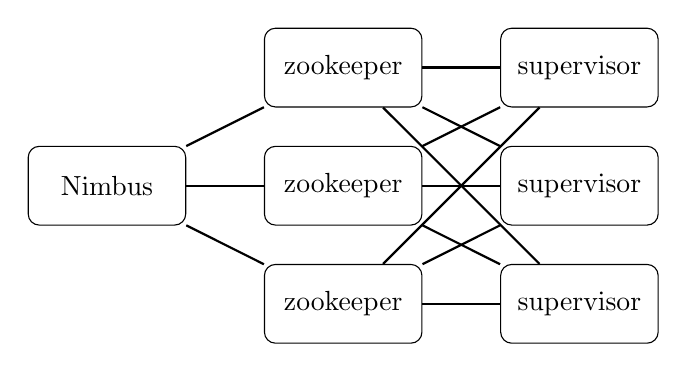
\begin{tikzpicture}
\tikzstyle{arrow} = [thick, -, >= stealth]
\tikzstyle{node} = [rectangle, rounded corners, minimum width = 2cm, minimum height=1cm,text centered, draw = black]
\node[node](Nimbus){Nimbus};
\node[node, right of = Nimbus, xshift = 2cm](zookeeper2){zookeeper};
\node[node, below of = zookeeper2, yshift = -0.5cm](zookeeper3){zookeeper};
\node[node, below of = zookeeper2, yshift = 2.5cm](zookeeper1){zookeeper};
\node[node, right of = zookeeper1, xshift = 2cm](supervisor1){supervisor};
\node[node, right of = zookeeper2, xshift = 2cm](supervisor2){supervisor};
\node[node, right of = zookeeper3, xshift = 2cm](supervisor3){supervisor};
\draw[arrow] (Nimbus)--(zookeeper1);
\draw[arrow] (Nimbus)--(zookeeper2);
\draw[arrow] (Nimbus)--(zookeeper3);
\draw[arrow] (zookeeper1)--(supervisor1);
\draw[arrow] (zookeeper1)--(supervisor2);
\draw[arrow] (zookeeper1)--(supervisor3);
\draw[arrow] (zookeeper2)--(supervisor1);
\draw[arrow] (zookeeper2)--(supervisor2);
\draw[arrow] (zookeeper2)--(supervisor3);
\draw[arrow] (zookeeper3)--(supervisor1);
\draw[arrow] (zookeeper3)--(supervisor2);
\draw[arrow] (zookeeper3)--(supervisor3);
\end{tikzpicture}
\caption{Storm架构示意图}
\label{storm_framework}
\end{center}
\end{figure}

\subsection{Spark}
Spark是一种通用的大数据计算框架,与Hadoop的MapReduce,Storm的
流式实时计算引擎十分相似。同时Spark也提供了大数据和机器学习方面的
框架,逐渐形成了大数据处理的一站式解决平台。

Spark的特点是支持大型,低延迟的数据处理方式。拓展了常用的MapReduce计算
模型。由于Spark支持在内存中进行计算,在必要时依赖硬盘进行复杂运算,因此
Spark比MapReduce更高效。

Spark是MapReduce的一种替代方案,兼容HDFS,Hive等存储方案,能够方便
地融入Hadoop的生态环境,以弥补MapReduce的不足。

\section{示例:人脸识别}


